\PassOptionsToPackage{dvipsnames,svgnames,x11names}{xcolor}
\documentclass[tikz,border=8pt]{standalone}
\usetikzlibrary{arrows.meta,positioning,calc,shapes,shadows,decorations.pathmorphing,shapes.geometric,backgrounds,decorations.markings,decorations.pathreplacing,decorations.text,fit,shapes.misc,shapes.arrows,matrix,bending,3d,chains,intersections,shapes.symbols,svg.path,shapes.multipart,snakes,shapes.callouts,angles,quotes}
\providecolor{gold}{RGB}{212,175,55}
\providecolor{silver}{RGB}{192,192,192}
\providecolor{bronze}{RGB}{205,127,50}
\providecolor{darkblue}{RGB}{0,0,139}
\providecolor{lightblue}{RGB}{173,216,230}
\providecolor{darkgreen}{RGB}{0,100,0}
\providecolor{lightgreen}{RGB}{144,238,144}
\providecolor{darkred}{RGB}{139,0,0}
\providecolor{navy}{RGB}{0,0,128}
\providecolor{skyblue}{RGB}{135,206,235}
\providecolor{beige}{RGB}{245,245,220}
\providecolor{cream}{RGB}{255,253,208}
\usepackage{amsmath}
\usepackage{amssymb}
\usepackage{fontawesome5}
\usetikzlibrary{fadings,shadows.blur,patterns,patterns.meta}



\usepackage{amsmath}
\usepackage{amssymb}
\usepackage{fontawesome5}
\usepackage{xcolor}

\providecolor{gold}{RGB}{212,175,55}
\providecolor{silver}{RGB}{192,192,192}
\providecolor{bronze}{RGB}{205,127,50}
\providecolor{darkblue}{RGB}{0,0,139}
\providecolor{lightblue}{RGB}{173,216,230}
\providecolor{darkgreen}{RGB}{0,100,0}
\providecolor{lightgreen}{RGB}{144,238,144}
\providecolor{darkred}{RGB}{139,0,0}
\providecolor{navy}{RGB}{0,0,128}
\providecolor{skyblue}{RGB}{135,206,235}
\providecolor{beige}{RGB}{245,245,220}
\providecolor{cream}{RGB}{255,253,208}

% --- COLOR DEFINITIONS ---
\definecolor{highlight}{RGB}{255, 152, 0}      % Orange Forecast
\definecolor{highlightdark}{RGB}{230, 120, 0}
\definecolor{highlightlight}{RGB}{255, 243, 224}
\definecolor{selectcolor}{RGB}{46, 125, 50}    % Success Green
\definecolor{selectlight}{RGB}{232, 245, 233}
\definecolor{infocolor}{RGB}{33, 150, 243}     % Standard Display Blue
\definecolor{retinacolor}{RGB}{103, 58, 183}   % High-DPI Purple
\definecolor{retinalight}{RGB}{149, 117, 205}  % Bright Purple Accent
\definecolor{terminalbg}{RGB}{30, 30, 30}      % Code Editor Dark Gray
\definecolor{terminalbar}{RGB}{48, 48, 48}     % macOS Window Title Bar
\definecolor{btnred}{RGB}{255, 96, 92}         % Window Close
\definecolor{btnyellow}{RGB}{255, 189, 68}     % Window Minimize
\definecolor{btngreen}{RGB}{0, 202, 78}        % Window Zoom
\definecolor{standsilver}{RGB}{215, 220, 225}  % Metallic Stand Highlight
\definecolor{standdark}{RGB}{160, 165, 170}    % Metallic Stand Shadow
\definecolor{screenbg}{RGB}{22, 25, 30}        % Deep Dark Screen Area
\definecolor{amber}{RGB}{255, 191, 0}
\definecolor{sky}{RGB}{135, 206, 235}

\begin{document}
\begin{tikzpicture}[
    box/.style={draw=black!20, fill=white, rounded corners=8pt, inner sep=12pt, blur shadow={shadow opacity=18, shadow blur steps=5, shadow yshift=-2pt}},
    mathnode/.style={box, text width=5.6cm, align=center, line width=1.2pt},
    arrow/.style={-Stealth, line width=2pt, rounded corners}
]

% --- ABSOLUTE BACKGROUND ---
\fill[white] (-16, -10) rectangle (16, 20);

% --- MAIN TITLE & SUBTITLE ---
\node[font=\Huge\bfseries, text=black!90] at (0, 18.5) {Executing the Forecast: Selecting from \texttt{srcset}};
\node[font=\Large\color{gray!80!black}] at (0, 17.7) {Combining forecasted CSS geometry with hardware pixel density.};

% --- CODE EDITOR WINDOW (MACOS STYLE) ---
% Container & Blur Shadow
\draw[fill=terminalbg, draw=black!70, rounded corners=6pt, line width=1pt, blur shadow={shadow opacity=30, shadow blur steps=6, shadow yshift=-3pt}]
    (-8.5, 13.5) rectangle (8.5, 16.5);

% Title Bar Clip
\begin{scope}
    \path[clip] (-8.5, 13.5) [rounded corners=6pt] rectangle (8.5, 16.5);
    \fill[terminalbar] (-8.5, 15.9) rectangle (8.5, 16.5);
    \draw[black!60, line width=0.75pt] (-8.5, 15.9) -- (8.5, 15.9);
    % Window Control Dots
    \fill[btnred] (-8.1, 16.2) circle (2.5pt);
    \fill[btnyellow] (-7.75, 16.2) circle (2.5pt);
    \fill[btngreen] (-7.4, 16.2) circle (2.5pt);
    % Title Bar Label
    \node[font=\scriptsize\ttfamily\bfseries, text=gray!40] at (0, 16.2) {index.html -- <img sizes="..." srcset="...">};
\end{scope}

% Syntax-Highlighted Code (Full <img> Context)
\node[font=\large\ttfamily, align=left, anchor=west] (srcset_text) at (-8.0, 14.7) {
    \textcolor{pink!80}{\textbf{<img}}\ \textcolor{orange!90}{\textbf{sizes}}=\textcolor{lime!90}{\textbf{"(max-width: 600px) 100vw, 33vw"}}\\
    \ \ \ \ \ \textcolor{orange!90}{\textbf{srcset}}=\textcolor{lime!90}{\textbf{"img-400.jpg}}\ \textcolor{cyan!80}{\textbf{400w}},\\
    \ \ \ \ \ \ \ \ \ \ \ \ \ \textcolor{lime!90}{\textbf{img-800.jpg}}\ \textcolor{cyan!80}{\textbf{800w}},\\
    \ \ \ \ \ \ \ \ \ \ \ \ \ \textcolor{lime!90}{\textbf{img-1200.jpg}}\ \textcolor{cyan!80}{\textbf{1200w}}\textcolor{lime!90}{\textbf{">}}
};

% --- FORECAST ENGINE MODULE ---
\draw[fill=white, draw=highlight, line width=2pt, rounded corners=8pt,
      blur shadow={shadow opacity=25, shadow blur steps=6, shadow yshift=-2pt},
      path picture={
          \draw[highlight!12, line width=0.5pt, step=0.35cm] (path picture bounding box.south west) grid (path picture bounding box.north east);
          \draw[highlight!50, line width=1.5pt] ($(path picture bounding box.north west)+(0.3,-0.1)$) -- ($(path picture bounding box.north west)+(0.1,-0.1)$) -- ($(path picture bounding box.north west)+(0.1,-0.3)$);
          \draw[highlight!50, line width=1.5pt] ($(path picture bounding box.south east)+(-0.3,0.1)$) -- ($(path picture bounding box.south east)+(-0.1,0.1)$) -- ($(path picture bounding box.south east)+(-0.1,0.3)$);
      }]
    (-5.5, 9.5) rectangle (5.5, 12.5);

\node[text width=10.5cm, align=center] at (0, 11.0) {
    \textbf{\color{highlight}\faCheckSquare\ From the previous \texttt{sizes} calculation:}\\[3pt]
    The engine successfully forecasted the CSS layout geometry to be exactly \textbf{400 CSS Pixels} wide.
};

% Connection Arrow: Code Editor to Forecast
\draw[-Stealth, line width=2pt, draw=highlight!80] (0, 13.5) -- (0, 12.5);

% Orthogonal Routing: Forecast Module to Monitors
\draw[-Stealth, line width=2pt, draw=highlight!85!infocolor, rounded corners=4pt]
    (0, 9.5) -- (0, 9.0) -| (-6.5, 8.5);
\draw[-Stealth, line width=2pt, draw=highlight!85!retinacolor, rounded corners=4pt]
    (0, 9.5) -- (0, 9.0) -| (6.5, 8.5);


% ==========================================
% --- STANDARD DISPLAY MONITOR (LEFT) ---
% ==========================================
% Monitor Stand Base & Neck
\fill[top color=standsilver, bottom color=standdark, draw=gray!60, rounded corners=1pt] (-6.9, 4.5) -- (-6.1, 4.5) -- (-6.25, 3.7) -- (-6.75, 3.7) -- cycle;
\filldraw[top color=standsilver!90!white, bottom color=standdark, draw=gray!60, rounded corners=2pt, blur shadow={shadow opacity=20, shadow blur steps=3, shadow yshift=-1pt}]
    (-7.8, 3.5) rectangle (-5.2, 3.7);

% Monitor Chassis Bezel
\draw[fill=gray!15, draw=gray!40, line width=1.5pt, rounded corners=10pt, blur shadow={shadow opacity=25, shadow blur steps=6, shadow yshift=-3pt}]
    (-10.5, 4.5) rectangle (-2.5, 8.5);

% Inner Dark Screen
\filldraw[fill=screenbg, draw=black!90, line width=1pt, rounded corners=4pt]
    (-10.2, 4.8) rectangle (-2.8, 8.2);
\fill[black!60] (-6.5, 8.35) circle (1.2pt); % Webcam

% Screen Content: Titles & Info
\node[font=\bfseries\color{infocolor}] at (-6.5, 7.8) {\faLaptop\ Standard Display};
\node[font=\small\color{white}] at (-6.5, 7.35) {Device Pixel Ratio (DPR): \textbf{\color{infocolor!30!white}1.0x}};
\node[font=\footnotesize\color{gray!35}, text width=7.5cm, align=center] at (-6.5, 6.95) {(1 hardware pixel = 1 CSS pixel)};

% Geometric DPR Visualizer (1x1 Grid)
\filldraw[fill=infocolor!25, draw=infocolor!80!white, line width=1.2pt] (-7.1, 5.25) rectangle (-5.5322,6.4763);
\node[font=\footnotesize\bfseries\color{infocolor!80!black}, scale=0.8] at (-6.2635,5.85) {1 HW Pixel};
\node[font=\scriptsize\bfseries\color{white}] at (-6.5, 4.95) {1 CSS px = 1 HW px};

% Standard Display Math Node
\draw[fill=white, draw=infocolor!60, rounded corners=8pt, line width=1.2pt, blur shadow={shadow opacity=18, shadow blur steps=5, shadow yshift=-2pt}]
    (-9.5, 0.8) rectangle (-3.5, 2.8);
\node[text width=5.6cm, align=center] at (-6.5, 1.8) {
    \textbf{Required Resolution:}\\[2pt]
    $400\text{px (layout)} \times 1.0\text{x (DPR)}$\\[4pt]
    \Large = \textbf{400 physical pixels}
};

% Connecting Arrow: Left Monitor Stand to Math Node 1
\draw[-Stealth, line width=2pt, draw=infocolor!80]
    (-6.5, 3.5) -- (-6.5, 2.8);


% ==========================================
% --- RETINA DISPLAY MONITOR (RIGHT) ---
% ==========================================
% Monitor Stand Base & Neck
\fill[top color=standsilver, bottom color=standdark, draw=gray!60, rounded corners=1pt] (6.1, 4.5) -- (6.9, 4.5) -- (6.75, 3.7) -- (6.25, 3.7) -- cycle;
\filldraw[top color=standsilver!90!white, bottom color=standdark, draw=gray!60, rounded corners=2pt, blur shadow={shadow opacity=20, shadow blur steps=3, shadow yshift=-1pt}]
    (5.2, 3.5) rectangle (7.8, 3.7);

% Monitor Chassis Bezel
\draw[fill=gray!15, draw=gray!40, line width=1.5pt, rounded corners=10pt, blur shadow={shadow opacity=25, shadow blur steps=6, shadow yshift=-3pt}]
    (2.5, 4.5) rectangle (10.5, 8.5);

% Inner Dark Screen
\filldraw[fill=screenbg, draw=black!90, line width=1pt, rounded corners=4pt]
    (2.8, 4.8) rectangle (10.2, 8.2);
\fill[black!60] (6.5, 8.35) circle (1.2pt); % Webcam

% Screen Content: Titles & Info
\node[font=\bfseries\color{retinalight}] at (6.5, 7.8) {\faApple\ High-DPI (Retina) Display};
\node[font=\small\color{white}] at (6.5, 7.35) {Device Pixel Ratio (DPR): \textbf{\color{retinalight!40!white}2.0x}};
\node[font=\footnotesize\color{gray!35}, text width=7.5cm, align=center] at (6.5, 6.95) {(4 hardware pixels = 1 CSS pixel (2x2 grid))};

% Geometric DPR Visualizer (2x2 Grid, Same Total Area)
\filldraw[fill=retinacolor!35, draw=retinalight!80!white, line width=1pt] (5.9, 5.85) rectangle (6.5, 6.45);
\filldraw[fill=retinacolor!35, draw=retinalight!80!white, line width=1pt] (6.5, 5.85) rectangle (7.1, 6.45);
\filldraw[fill=retinacolor!35, draw=retinalight!80!white, line width=1pt] (5.9, 5.25) rectangle (6.5, 5.85);
\filldraw[fill=retinacolor!35, draw=retinalight!80!white, line width=1pt] (6.5, 5.25) rectangle (7.1, 5.85);
\draw[retinalight, line width=1.5pt] (5.9, 5.25) rectangle (7.1, 6.45);
\node[font=\tiny\bfseries\color{white}] at (6.2, 6.15) {HW};
\node[font=\tiny\bfseries\color{white}] at (6.8, 6.15) {HW};
\node[font=\tiny\bfseries\color{white}] at (6.2, 5.55) {HW};
\node[font=\tiny\bfseries\color{white}] at (6.8, 5.55) {HW};
\node[font=\scriptsize\bfseries\color{white}] at (6.5, 4.95) {1 CSS px = 4 HW px};

% Retina Display Math Node
\draw[fill=white, draw=retinacolor!60, rounded corners=8pt, line width=1.2pt, blur shadow={shadow opacity=18, shadow blur steps=5, shadow yshift=-2pt}]
    (3.5, 0.8) rectangle (9.5, 2.8);
\node[text width=5.6cm, align=center] at (6.5, 1.8) {
    \textbf{Required Resolution:}\\[2pt]
    $400\text{px (layout)} \times 2.0\text{x (DPR)}$\\[4pt]
    \Large = \textbf{800 physical pixels}
};

% Connecting Arrow: Right Monitor Stand to Math Node 2
\draw[-Stealth, line width=2pt, draw=retinacolor!80]
    (6.5, 3.5) -- (6.5, 2.8);


% ==========================================
% --- SELECTED IMAGE FILE 1 (LEFT) ---
% ==========================================
% Realistic Folded Document Path (Wider 8-unit geometry)
\path[fill=selectcolor!5, draw=selectcolor, line width=1.8pt, rounded corners=2pt, blur shadow={shadow opacity=18, shadow blur steps=4, shadow yshift=-2pt}]
    (-10.5, -4.5) -- (-2.5, -4.5) -- (-2.5, -1.5) -- (-4.0, 0.0) -- (-10.5, 0.0) -- cycle;
% Folded Corner Flap
\path[fill=selectcolor!15, draw=selectcolor, line width=1.2pt]
    (-4.0, 0.0) -- (-4.0, -1.5) -- (-2.5, -1.5) -- cycle;

% Header
\node[font=\normalsize\bfseries\color{selectcolor}, anchor=north] at (-6.5, -0.2) {\faFileImage\ Selected File};

% Miniature Image Thumbnail Badge (Landscape with Sun & Mountains)
\draw[fill=sky!15, draw=selectcolor!40, rounded corners=2pt] (-10.2, -3.5) rectangle (-8.2, -1.5);
\begin{scope}
    \path[clip] (-10.2, -3.5) [rounded corners=2pt] rectangle (-8.2, -1.5);
    \fill[orange!85] (-8.8, -2.0) circle (0.22cm);
    \fill[selectcolor!75!black] (-10.3, -3.5) -- (-9.4, -2.3) -- (-8.5, -3.5) -- cycle;
    \fill[selectcolor!55!black] (-9.0, -3.5) -- (-8.4, -2.5) -- (-7.9, -3.5) -- cycle;
\end{scope}

% Text Details
\node[font=\large\ttfamily\bfseries, text=black!90, anchor=west] at (-7.8, -2.0) {img-400.jpg};
\node[font=\footnotesize\color{black!70}, anchor=west, text width=4.2cm, align=left] at (-7.8, -2.8) {(A perfect 1:1 pixel match)};

% Arrow: Math 1 to File 1
\draw[-Stealth, line width=2pt, draw=selectcolor]
    (-6.5, 0.8) -- (-6.5, 0.0);


% ==========================================
% --- SELECTED IMAGE FILE 2 (RIGHT) ---
% ==========================================
% Realistic Folded Document Path (Wider 8-unit geometry)
\path[fill=selectcolor!5, draw=selectcolor, line width=1.8pt, rounded corners=2pt, blur shadow={shadow opacity=18, shadow blur steps=4, shadow yshift=-2pt}]
    (2.5, -4.5) -- (10.5, -4.5) -- (10.5, -1.5) -- (9.0, 0.0) -- (2.5, 0.0) -- cycle;
% Folded Corner Flap
\path[fill=selectcolor!15, draw=selectcolor, line width=1.2pt]
    (9.0, 0.0) -- (9.0, -1.5) -- (10.5, -1.5) -- cycle;

% Header
\node[font=\normalsize\bfseries\color{selectcolor}, anchor=north] at (6.5, -0.2) {\faFileImage\ Selected File};

% Miniature Image Thumbnail Badge (Landscape with Sun & Mountains)
\draw[fill=sky!15, draw=selectcolor!40, rounded corners=2pt] (3.0, -3.5) rectangle (5.0, -1.5);
\begin{scope}
    \path[clip] (3.0, -3.5) [rounded corners=2pt] rectangle (5.0, -1.5);
    \fill[orange!85] (4.4, -2.0) circle (0.22cm);
    \fill[selectcolor!75!black] (2.9, -3.5) -- (3.8, -2.3) -- (4.7, -3.5) -- cycle;
    \fill[selectcolor!55!black] (4.2, -3.5) -- (4.8, -2.5) -- (5.3, -3.5) -- cycle;
\end{scope}

% Text Details
\node[font=\large\ttfamily\bfseries, text=black!90, anchor=west] at (5.3, -2.0) {img-800.jpg};
\node[font=\footnotesize\color{black!70}, anchor=west, text width=4.2cm, align=left] at (5.3, -2.8) {(Double resolution for crisp rendering)};

% Arrow: Math 2 to File 2
\draw[-Stealth, line width=2pt, draw=selectcolor]
    (6.5, 0.8) -- (6.5, 0.0);


% ==========================================
% --- CONCLUSION PLACARD ---
% ==========================================
\draw[fill=black!4, draw=black!25, line width=1.2pt, rounded corners=8pt,
      blur shadow={shadow opacity=15, shadow blur steps=4, shadow yshift=-2pt}]
    (-9.5, -9.2) rectangle (9.5, -5.8);

\node[text width=18cm, align=center, font=\large] at (0, -7.5) {
    \textbf{\color{amber!80!black}\faLightbulb\ The Power of the Forecast:}\\[4pt]
    Because we explicitly forecast the geometry in HTML, the Preload Scanner can perform this math \textbf{instantly}, selecting and downloading the exact right image file before the CSS parser has even finished reading the stylesheet!
};

\end{tikzpicture}
\end{document}
